\chapter{\color{oxfordblue} Theoretical Particle Physics}\label{chap-theory}
\textit{Particle Physics is the field of science dedicated to the study of the fundamental elements of matters and of their interactions. Nature at this scale is best represented by an intricate connexion between particles, the fundamental components of matter, and their interactions, themselves represented by particles. This framework is encapsulated into a mathematical foundation called quantum field theory. A major scientific achievement of the second half of the $20^{\text{th}}$ century is the elaboration of the so-called Standard Model of Particle Physics, a unified patchwork of theories describing all known elementary particles and three of the four fundamental interactions affecting them. This chapter reviews relevant elements of the theory to contextualise the work presented in this thesis.}

\section{The Standard Model of Particle Physics}\label{Section:SM}
To date, the \gls{sm} has been the most successful theory in describing the constituents and the dynamics of matter \cite{SMphysics}. The \gls{sm} stands at the centre of theoretical particle physics, ellaborated by combining different successful theories of quantum mechanis and special relativity in the second part of the 20$^{th}$ century. These different exploits have led to a total of 55 Nobel Prizes. The \gls{sm} is often hailed as the most successful theory of science, with the unique ability to predict properties of the Universe to a staggering degree of precision: most famously, the anomalous magnetic dipole moment predictions is in agreement with measurements to up to 10 significant decimals \cite{PhysRevA.83.052122}. The \gls{sm} is expressed in the language of the dynamics of quantised fields, or \gls{qft}. These fields play two roles: describing matter itself (\textit{fermions}, such as the electron) and the different interactions (\textit{bosons}, such as the $W$ and the famous Higgs boson $H$) governing how this matter interacts under the electromagnetic, weak, and strong interactions. Particles are the results of local excitations of quantised fields that are defined as operator-values distributions over spacetime. Figure \ref{particlesSM} displays the fundamentals particles of the \gls{sm}. \\

\begin{figure}[!h]
    \centering
    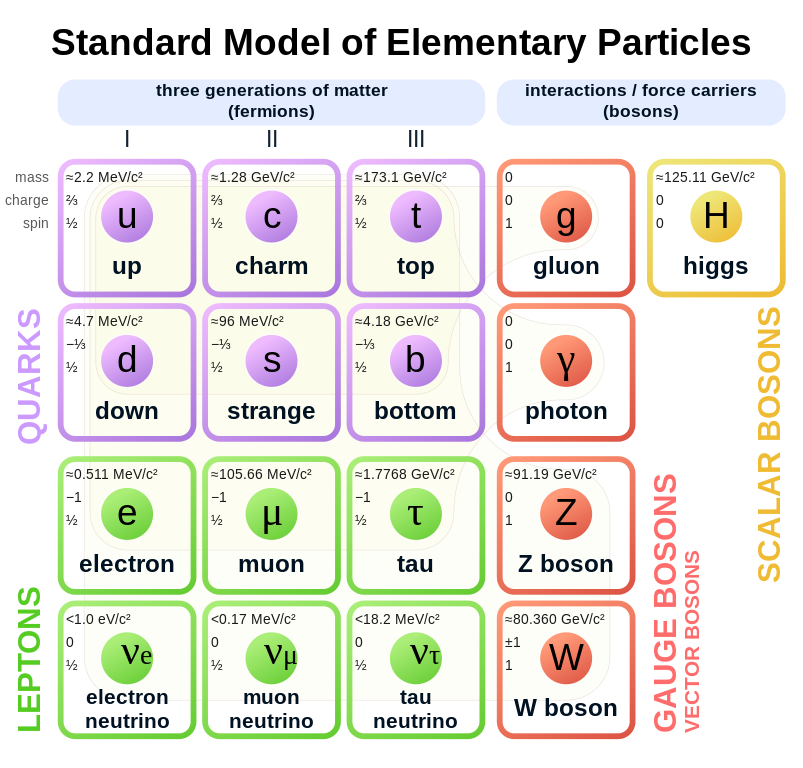
\includegraphics[width=0.8\textwidth]{Images/Theory/particlesSM.png} % TODO update to a more up to date. % TODO update the ref
    \caption[Particles in the SM]{Elementary particles of the Standard Model \cite{tableSMWiki}. Elementary fermions (quarks on top, lepton on the bottom) are listed in the three left columns and elementary bosons in the two right ones, the gauge bosons in the first column and the Higgs scalar boson in the last one. The mass, electrical charge, and spins of the particles are indicated.}
    \label{particlesSM}
\end{figure}

Particles are separated based on their intrinsic angular momentum or \textit{spin}, with half-spin particles following the Fermi-Dirac statistics called \textit{fermions}, and integer-spin particles called \textit{bosons} following the Bose-Einstein statistics. The elementary fermions are evenly split into 6 quarks and 6 leptons, with only the first generation of each being stable. The distinction between these two types stems from the different quantum numbers categorising them. Quarks carry a fractional electromagnetic charge as well as a colour charge making them sensitive to the strong interaction. On the contrary, leptons are colour-neutral and either have an electrical charge of -1$e^+$, in units of the anti-electron (positron) charge, or are neutral. The charged leptons include the electron $e^-$ - the lightest and only stable one -, the muon $\mu^-$, and the tau $\tau^-$. The neutral leptons are called neutrinos, with one neutrino $\nu_\ell$ associated per charged lepton $ell$, e.g., the electron-neutrino $\nu_e$. For the quarks, the electromagnetic charge is fractional, dividing them evenly between \textit{up}-type quarks with charge +$\frac{2}{3}$ consisting of the up $u$, charm $c$, and top $t$ flavours, and the \textit{down}-type quarks with charge -$\frac{1}{3}$ and the flavours down $d$, strange $s$, and bottom $b$. To every particle corresponds an \textit{anti}particle, with the same quantum numbers except for the electrical charge that changes sign. \\

The kinematics and dynamics of the fields representing the particles in the theory are expressed through a Lagrangian density $\mathcal{L}$, a spacetime discretisated element of the general Lagrangian. Symmetries of the Lagrangian density play an essential role as they define conserved quantities through Noether's theorem. The construction of the \gls{sm} Lagrangian id dictated by the expression of these symmetries to satisfy the experimentally observed conserved quantities, such as the electromagnetic charge. Two types of symmetries can be considered: global ones that are valid across spacetime and local ones, the so-called gauge symmetries valid for localised transformations. The \gls{sm} Lagrangian must satisfy the global Poincaré symmetry, encapsulating the symmetry required for special relativity, and a local non-Abelian $SU(3)_C \otimes SU(2)_L \otimes U(1)_Y$ gauge symmetry. Non-Abelian groups are such that their generators do not commute. The Lagrangian density of a field $\psi$ is a function of $\psi$ and its spacetime partial derivative $\partial_{\mu} \psi$, where $\mu$ indexes the time and space dimenions in the 4-vector formalism. The full \gls{sm} Lagrangian $\mathcal{L}_{\text{SM}}$ can be decomposed into 4 terms:
\begin{equation}\label{eq-SMGlobal}
    \mathcal{L}_{\text{SM}} = \mathcal{L}_{\text{EW}} + \mathcal{L}_{\text{QCD}} + \mathcal{L}_{\text{Higgs}} + \mathcal{L}_{\text{Yukawa}}.
\end{equation}
These different terms represent different effects encoded within the unified framework of the \gls{sm}. Three of the four known interactions of nature are encapuslated in the \gls{sm}: the strong, the electromagnetic, and the weak forces, with the gravitational force considered aside due to the weakness of its influence at sub-atomic scales. The mediators of the three included interactions are the gauge bosons, spin 1 particles with different properties arising from the nature of the interaction they carry. The electromagnetic and weak force have been successfully unified as a single \gls{ew} interaction, while the theory of the strong force is \gls{qcd}. One essential element in the \gls{sm} is the so-called Higgs interaction, a special force through which some gauge bosons acquire mass. This Higgs interaction is underpinned by a Higgs field, an excitation of which is called a Higgs boson $H$. Interactions between the Higgs field and quark can be introduced to assign masses to the latter through Yukawa couplings. The latter part of this thesis is dedicated to a measurement of such couplings to $b$- and $c$-quarks. The different interactions and their respective gauge bosons are further reviewed in this chapter.

\subsection{Quantum Electrodynamics}\label{subsec-QED}
\glsfirst{qed} is the theory underpinning the behaviour of free fermions and their electromagnetic interactions, for which the gauge carried are the photons. Fermions are represented by a Dirac spinor field $\psi(x)$ defined over spacetime $x$. The Dirac equation of quantum mechanics is a first order partial derivative equation modelling the free dynamics of such a spin-$\frac{1}{2}$ fermion with:
\begin{equation}\label{eq-dirac}
    (i\gamma^{\mu} \partial_{\mu} - m) \psi = 0,
\end{equation}
where $\gamma^{\mu}$ are the Dirac $\gamma$-matrices generalising the Pauli spin matrices to spacetime dimension, and the Einstein notation is adopted, summing over indices repeated as covariant and contravariant. For clarity, any contraction $\gamma^{\mu} \partial_{\mu}$ is denoted as $\cancel{\partial}$. A Lagragian density can be constructed to result in the dynamics described by Equation \ref{eq-dirac} through application of Euler-Lagrange:
\begin{equation}\label{eq-diracLag}
   \mathcal{L}_{\text{Dirac}} = \bar{\psi} (i \cancel{\partial}- m) \psi,
\end{equation}
Such a Lagrangian models the free dynamics of any spin-$\frac{1}{2}$ fermion, such as an electron $e^-$. Electrons have a $q = -1$ charge that is conserved by every known interactions. This conservations must be the result of a symmetry: the Dirac Lagrangian must be made invariant under a local gauge $U(1)$ transformation:
\begin{equation}\label{eq-GaugeU1}
    \psi \rightarrow \psi' = e^{-iq\alpha(x)} \psi ,
\end{equation}
which corresponds to a rotation in the complex spacetime by a phase $q\alpha(x)$. For the Lagrangian of Equation \ref{eq-diracLag} to satisfy this symmetry, the partial derivative $\partial_{\mu}$ must be replaced by the \textit{gauge covriant derivative $D_{\mu}$}:
\begin{equation}\label{eq-GaugeU1}
    \partial_{\mu} \rightarrow \partial_{\mu} + iqA_{\mu},
\end{equation}
where a new vector field $A\mu$ is introduced and required to transform under the $U(1)$ symmetry as $A_{\mu} \rightarrow A'_{\mu} = A_{\mu} + \partial_{\mu} \alpha(x)$. The elegance of this approach is the possibility to give this fauge field $A_{\mu}$ its own dynamic, modifying the Lagrangian of Equation \ref{eq-diracLag} into the \gls{qed} Lagrangian: \[ \mathcal{L}_{\text{QED}} = \bar{\psi} (i \cancel{\partial}- m) \psi + q \bar{\psi} \cancel{A} \psi - \frac{1}{4} F_{\mu\nu} F^{\mu\nu} \]
\begin{equation}
    \mathcal{L}_{\text{QED}} = \bar{\psi} (i \cancel{D}- m) \psi - \frac{1}{4} F_{\mu\nu} F^{\mu\nu}
\end{equation}
where $F_{\mu\nu} = \partial_{\mu} A_\nu - \partial_\nu A_{\mu} $ is the electromagnetic field tensor. The last term introduces a kinetic term for the gauge field and the interaction between the fermion $\psi$ and the gauge field $A$ is represented by the term combining them. In the present case, the charge $q$ is the conserved quantity of the gauge symmetry, which required the introduction of a new gauge field $A_\mu$ that can be interpreted as the photon field and given the dynamic of the electromagnetic interaction through $F_{\mu\nu}$. Fermionic fields can be introduced in this approach for the different known fermions, $\psi_e$, $\psi_{\mu}$, $\psi_u$, $\psi_c$, etc. Their interactions with $A_\mu$ defining each time a unique conserved electromagnetic charge $q_e$, $q_{\mu}$, $q_u$, $q_c$, etc.  This procedure is however general: the gauge invariance of a Lagrangian introduces a spin-1 gauge vector boson. The required $U(1)$ invariance forbids the presence of mass terms of the form $m^2 A^{\mu} A_{\mu}$, seemingly condemning the gauge bosons to be massless. 

\subsection{Electroweak Sector}
The weak force is described by two massive gauge vector bosons: the $W^{\pm}$ of mass $m_W \approx 80.4$ GeV\footnote{The unit system adopted throughtout this thesis is to set the speed of light in vacuum $c$ at 1, leading to masses expressed in GeV. To convert to mass units, one simply needs to divide by the standard unit $c^2$.} and the $Z^0$ of mass $m_Z \approx 91.2$ GeV. This apparent contradiction with the massless requirements of a $U(1)$ symmetry is elegantly solved by the Brout-Englert-Higgs mechanism \cite{Englert:1964et,  PhysRevLett.13.508}. This mechanism, described in the next section, is applied to a joint expression of the electromagnetic and weak forces known as \glsfirst{ew} theory in the Glashow-Weinberg-Salam (GWS) model \cite{GLASHOW1961579, PhysRevLett.19.1264, Salam:1968rm}. The fundamental symmetry group the theory is built upon is the non-Abelian $SU(2)_L \otimes U(1)_Y$, where $SU(2)_L$ is the weak isospin and $U(1)_Y$ the weak hypercharge. A local $SU(2)$ transformation acts as:
\begin{equation}\label{eq-GaugeSU2}
    \psi \rightarrow \psi' = e^{i g \alpha^a(x) T^a } \psi,
\end{equation}
where $T^a = \sigma^a / 2$ are the generators of the $SU(2)_L$ group, built from the $\sigma^a$ Pauli matrices ($a = 1, 2, 3)$. Each generator corresponds to a gauge field. The gauge field linked to $SU(2)_L$ leads to covariant derivative, simularly to Equation \ref{eq-GaugeSU2}, to ensure gauge invariance as expressed by
\begin{equation}\label{eq-GaugeSU2}
   D_{\mu}  = \partial_{\mu} + igT_a W_{\mu}^a,
\end{equation}
with three gauge fields $W_{\mu}^1$, $W_{\mu}^2$, $W_{\mu}^3$ with interaction strength $g$. The particularity of the weak interaction is that the charged current interactions described by the symmetry group $SU(2)_L$ only apply to left-handed $L$ particles states and not the right-handed $R$. Consequently, fermionic fields are decomposed into \[\psi = \psi_L + \psi_R\] with left-and right-handed particles represented by isospin doublets. The weak isospin $I_W$ charge of left-handed particles is $I_W = 1/2$, with a third component $I_W^3 = \pm  1/2$. For the right-handed part, $I_W = 0$ with $I_W^3 = 0$, decoupling it from the gauge bosons $W_{\mu}^a$. Physically, the observed weak charge current interaction corresponding to the $W^{\pm}$ bosons are the linear combinations of gauge fields:
\begin{equation}
    W_{\mu}^{\pm} = \frac{1}{\sqrt{2}} \left(W_{\mu}^{1} \mp W_{\mu}^{2} \right)
\end{equation}
These $W$ bosons only couple to left-handed particles, but an experimentally observed $Z$ boson couples to both left- and right-handed particles. This represented by the additional $U(1)_Y$ symmetry of the weak interaction in the \gls{sm}, with weak hypercharge $Y$, coupling $g'$, and an additional gauge field $B_{\mu}$. The weak hypercharge is \[Y = 2 (Q - I_W^3),\] with $Q$ the electromagnetic charge. The total covariant derivative of the electroweak sector of the \gls{sm} is therefore expressed by the GSM model as 
\begin{equation}\label{eq-GaugeEW}
    D_{\mu}  = \partial_{\mu} + ig T_a W_{\mu}^a + ig' \frac{Y}{2} B_{\mu}. % TODO should these be the g and g
\end{equation}
where $W_{\mu}^a$ and $B_{\mu}$ are respectively the $SU(2)_L$ and $U(1)_Y$ gauge bosons. The GSM model re-expresses the electromagnetic photonic field $A_\mu$ and the $Z$-boson field $Z_{\mu}$ as a linear combination of $B_{\mu}$ and $W_{\mu}^3$ depending on the \textit{weak mixing angle} $\theta_W$, a fundamental parameter of the \gls{sm} such that:
\begin{equation}\label{eq-weakmixangle}
    \cos\theta_W = \frac{g}{\sqrt{g^2 +g'^2}}.
\end{equation}
This establishes a connexion between the coupling strengths of the weak interaction and the electromagnetic interaction coupling $e$ as \[e = g \sin \theta_W = g' \sin\theta_W \cos\theta_W.\] The intrinsic strength of the weak interactions is indeed of similar ordar to that of the electromagnetic interaction but is weak in apparance due to its gauge bosons being massive. The weak force is the only known fundamental interaction to violate parity conservation. Neutrinos can only interact throught the weak force, which can itself only apply to left-handed particles. As a result, there are no right-handed neutrinos in the \gls{sm}. \\

A significant achievement of modern particle physics is the unification of interactions that are perceived as different at low-energies. The problem of the measured mass of the vector gauge bosons remains . Additionaly, the split of fermionic fields into a left- and right-handed componets lead the mass terms to violate the gauge invariance. Both issues are resolved by the mechanisms of the next two sections.

\subsection{The Brout-Englert-Higgs Mechanism}
The Brout-Englert-Higgs mechanism, abbreviated $BEH$ henceforth, offers a solution to introduce mass terms to the gauge fields $W_{\mu}^{\pm}$ and $Z_{\mu}$. It introduces a new scalar Higgs field, permeating the Universe. The field is mathematically defined as a weak isospin doublet, with a neutral component $\phi^0$ and a charged one $\phi^+$. They are jointly expressed as complex scalar field with 4 degrees of freedom:
\begin{equation}
\phi = \begin{pmatrix}
    \phi^+\\ 
    \phi^0
\end{pmatrix} = \frac{1}{2} \begin{pmatrix}
    \phi_1 + i\phi_2 \\ 
    \phi_3 + i\phi_4
\end{pmatrix}
\end{equation}
This complex scalar field is made to interact with the electroweak gauge fields as 
\begin{equation}\label{eq-HiggsLag}
    \mathcal{L_{\text{Higgs}}} = (D_{\mu}\phi)^{\dagger} (D^{\mu}\phi) - V(\phi),
 \end{equation}
where the first term described the kinetic of the $\phi$ and the second term is the Higgs potential energy:
\begin{equation}\label{eq-HiggsLag}
 V(\phi) = - \mu^2  \phi^{\dagger} \phi + \lambda (\phi^{\dagger} \phi)^2.
\end{equation}
where the expression of this potential is constrained by the need for the theory to be renormalisable. Two scalars constants govern the Higgs potential: $\mu$ and $\lambda$ describing, respectively, the quadratic and quartic interaction of the complex Higgs field $\phi$. The former manifests the interaction with the gauge bosons, while the latter introduces self-interactions. The minimum of this potential corresponds to the vacuum state. The requirement that the vacuum be stable demands $\lambda > 0$. For a positive $\mu^2 > 0$, a degenerate minimum is found at field values such that
\begin{equation}\label{eq-HiggsLag}
    \phi^{\dagger} \phi  = \frac{1}{2} (\phi_1^2 + \phi_2^2 + \phi_3^2 + \phi_4^2) = \frac{- \mu^2}{2\lambda} = \frac{v^2}{2}
\end{equation}
introducing in the last equality the so-called \textit{vacuum expectation value} $v = \sqrt{\frac{|\mu^2|}{\lambda}}$ of the field $\phi$. This infinite degeneracy of the Higgs potential minimum states underlines a special $SU(2)$ symmetry such that $\phi^{\dagger} \phi = v^2/2$. Through \textit{spontaneous symmetry breaking}, the BEH mechanism crumbles this degeneracy into one single vacuum state typically chosen by setting the components $\phi_1 = \phi_2 = \phi_4 = 0$ and $\phi_3 = v$ so that the vacuum expactation is simply
\begin{equation}
\langle0|\phi|0 \rangle = \frac{1}{\sqrt{2}} \begin{pmatrix}
        0\\ 
        v
    \end{pmatrix}.
\end{equation}
The breaking of the symmetry enforces \[ SU(2)_L \otimes U(1)_Y \rightarrow U(1)_Q,\] with the final vacuum state correctly set as chargeless.

Expanding the full field dynamic around the chosen vacuum state with a particular gauge choice to absord unphysical Goldstone fields into the vector fields called \textit{unitarity gauge} \cite{PhysRevD.7.1068}, the expansion can be simplified to 
\begin{equation}
    \phi = \frac{1}{\sqrt{2}} \begin{pmatrix}
            0\\ 
            v + h(x)
        \end{pmatrix},
\end{equation}
where $h$ is the real neutral Higgs scalar field. Introducing this expression into the Higgs Lagrangian of Equation~\ref{eq-HiggsLag} gives
\begin{equation}\label{eq-fullHiggs}
    \begin{split}
        \mathcal{L}_{\text{Higgs}} = & \,\frac{1}{2} (\partial_\mu h)(\partial^\mu h) + \frac{\mu^2}{2}(v+h)^2  - \frac{\lambda}{16}(v+h)^4 \\
        &+ \frac{1}{4} g^2 (W_{\mu}^+W^{\mu-})(v+h)^2 + \frac{g^2_W + {g'}^2}{8}(Z_{\mu}Z^{\mu})(v+h)^2 
    \end{split}
\end{equation}
where one can clearly identify mass terms for the physical gauge fields $W_{\mu}^{\pm}$ and $Z_\mu$ in the last line, but not for $A_{\mu}$ as required from observations that photons are massless. The vector gauge bosons masses are:
\begin{equation}
    m_W = \frac{v}{2} g , \, m_Z = \frac{v}{2}\sqrt{g^2 +g'^2} 
\end{equation}
or equivalenty expressing the mass of the $Z$-boson in terms of the $W$-boson mass \[m_Z = \frac{m_W}{\cos\theta_W}.\] The Higgs field is massive\footnote{This requires to isolate the terms in $h^2$ in Equation \ref{eq-fullHiggs}.} with mass \[m_H = \sqrt{2|\mu^2|}.\]
The BEH mechanism elegantly assigns mass to the gauge vector boson, with the photon remaining massless and the addition of the Higgs boson $H$ as a massive elementary particle. Furthermore, the introduction of the related Higgs field permits the expression of mass terms for the fermions in the standard model, as explained in Section~\ref{subset-yukint} on Yukawa interactions. 

\subsection{Quantum Chromodynamics}
The strong interaction is described by the theory of \textit{\glsfirst{qcd}}, underpinned by an $SU(3)_C$ symmetry with conserved quantum number called \textit{colour}. The only particles having a colour charge in the \gls{sm} are quarks and gluons $g$, the gauge mediators of the strong interactions. There are three colour charges typically labelled \textit{red}, \textit{blue}, and \textit{green}, each coming into its direct or anti-colour (e.g., anti-red). Quarks carry one such charge and gluons two. Similarly to the electroweak sector, the symmetry leads to a covariant derivative under the $SU(3)_C$ group of
\begin{equation}\label{eq-GaugeQCD}
    D_{\mu}  = \partial_{\mu} + ig_s \lambda_a G_{\mu}^a. % TODO should these be the g and g
\end{equation}
where the coupling constant $g_s$ of the strong interaction is often re-expressed as $\alpha_s = \frac{g_s}{4\pi}$, and the generator of the $SU(3)_C$ group are the set of eight $\lambda_a$ Gell-Mann matrices. The gauge field introduced here are the $G_{\mu}^a$ corresponding to the associate mediator of the strong field: the gluons $g$. Gluons carry 2 colour charges, leading to the 8 Gell-Mann matrices $\lambda^a$ and 8 gauge vector fields $G_{\mu}^a$. The generators of the $SU(3)_C$ group do not commutate: \[ [\lambda^a, \lambda^b] = i f^{abc} \lambda^c,\] where $f^{abc}$ are the $SU(3)_C$ structure constants.  Similarly to the electromagnetic strength tensor, strength tensors are built from the gluon fields as \[G_{\mu\nu}^a = \partial_{\mu} G_{\nu}^a   - \partial_{\nu} G_{\mu}^a - g_s f^{abc} G_{\mu}^b G_{\nu}^c.\]
This leads to a total \gls{qcd} Lagrangian of:
\begin{equation}\label{eq-QCDLag}
    \mathcal{L}_{\text{QCD}} = -\frac{1}{4} G_{\mu\nu}^a G^{\mu\nu}_a + \sum_{k} \bar{\psi}_k (i \cancel{D} - m_k) \psi_k,
\end{equation}
where $\psi_k$ are the six quarks fields, one per flavour, transforming as an $SU(3)_C$ triplet with one component per colour quantum number. Cubic and quartir terms in the gluon gauge fields $G_{\mu}^a$ are included, introducing self interaction of gluons. The non-commutation of the $SU(3)_C$ generators means the $SU(3)_C$ part of the \gls{sm} is non-Abelian group, and therefore a case of a Yang-Mills theory requiring this self-interacting gauge fields \cite{PhysRev.96.191}. \\

Like every coupling constant, $\alpha_s$ varies with energy. At low energies, the interaction is so strong that perturbative calculation breaks and the behaviour of \textit{colour confinement} is observed: any attempt to isolate a quark requires so much energy that a quark-antiquark pair is spontaneously produced. The strength of this interaction explains it short propagation distance despite the fact its gluonic mediatiors are massless. At higher energies $\sim 100$ GeV, asympotic freedom and perturbative calculations are possible thanks to the smallness of the coupling strength. This typically requires higher-order corrections for calculation to converge, with some terms, such as quark self-energy loops, diverging to infinity. This type of diverge is  called \textit{ultraviolet divergence}, and it is fixed by renormalising fields and parameters so that the divergence are absorbed away. This correction requires two parameters to arbitrarily define the scale of the process: the \textit{renormalisation scale} $\mu_R$ and \textit{factorisation scale} $\mu_F$ \cite{collins2004factorization}. The former is introduced to deal with ultraviolet divergences in the running of $\alpha_s$. The latter addresses the so-called \textit{infrared divergences} due to massless particles radiating further massless particles at low-energies by entering the parton distribution and fragmentation functions, introduced latter in this chapter.\\

Quarks must combine to form colour-less aggregate of matters called hadrons, with either a 2-quark system combining a quark and an antiquark into a \textit{meson}, or a 3-quark system forming a \textit{baryon} of which the proton ($uud$, $q_p = +1$) and the neutrons ($udd$, $q_n = 0$) are prime examples. The content of hadrons are called partons. The process leading to the neutralisation of the colour-charge of an asymptotically freed quark is called \textit{hadronisation}.\\

\subsection{Yukawa Interactions}\label{subset-yukint}
In the \gls{qcd} Lagrangian of Equation~\ref{eq-QCDLag}, the introduction of the mass terms for the quarks breaks the gauge invariance of the theory to $SU(2)_L \otimes U(1)_Y$ and must be therefore further modified. The masses of all fermions can however be included in the \gls{sm} by introducing so-called Yukawa interactions between the Higgs and fermionic fields. Such terms are expressed as the following Lagrangian:
\begin{equation}\label{eq-YukLag}
    \mathcal{L}_{\text{Yukawa}} = - \sum_{f} 
    -\frac{y_f}{\sqrt{2}} \bar{\psi}_f (v + h) \psi_f,
\end{equation}
where $\psi_f$ are the fermionic fields and the fundamental \textit{Yukawa coupling} parameters $y_f = \sqrt{2} \frac{m_f}{v}$ for each flavour of fermion $f$ are introduced as coupling strengths. Picking the $v$ component in the sum in parenthesis gives a clear mass term to the fermion, with the $h$ terms leading to Higgs-fermion interactions. The vacuum expectation value plays the role of a mass scale setting, with Yukawa coupling refining the specific strength for each fermionic species. For the quark sector, a futher correction is required as the weak interaction eigenstate basis is different from the mass basis in which physical particles are detected. The transformation from the mass eigenstates basis is specified by the complex unitary \textit{\gls{ckm} matrix} \cite{Tanabashi:2018oca}:
\begin{equation}
    V_{CKM} = \begin{pmatrix}
            V_{ud} & V_{us} & V_{ub}\\ 
            V_{cd} & V_{cs} & V_{cb}\\ 
            V_{td} & V_{ts} & V_{tb}\\ 
        \end{pmatrix},
\end{equation}
where the probability of a transition $p \rightarrow q$ is given by the magnitude $|V_{pq}|^2$ of the associated element. Through this quark mixing matrix, weak charged currents interaction allows for flavour-changing processes through charged currents interactions. The matrix is almost diagonal, hence transitions between quarks of the same generation are preferred (e.g., $t \rightarrow b$ preferred over $t \rightarrow d$).

\subsection{Experimental Phenomenology}
The experimental process to observe the Higgs bosons at the \gls{lhc} is to collide two protons beams head-on, as described in Chapter~\ref{chapter-ATLAS}. The accelerator is primarily designed to achieve these measurements, targeting different production and decay channels. Protons are composite particules (hadrons) and, at high energies, the main \textit{hard-scattering} interaction is beteen components of the protons called \textit{partons}. These partons are primarily the \textit{valence} quarks ($uud$ for a proton) but also contribution from \textit{sea} quarks, as well as gluons and photons present within the hadron due to quantum interactions. In a two protons $pp$ collision, two interacting partons $ab$ will undergo the main event $ab \rightarrow X$, with the rest of the activity assigned to the so-called \textit{\gls{ue}}. The cross-section for the process $pp \rightarrow X$ can be factorised into \cite{collins2004factorization}: 
\begin{equation}
\sigma_{pp\rightarrow X} \sum_{a,b} \int_0^1 dx_a \int_0^1 dx_b f_a(x_a, \mu_F) f_b(x_b, \mu_F) \int d\sigma_{ab\rightarrow X}\left(x_aP_a, x_bP_b, \mu_R \mu_F \right),
\end{equation}
where the $f_i(x_i, \mu_F)$ are \textit{\gls{pdf}} giving the probability for a parton $i$ to undergo a hard scattering with momentum $p_i = x_i P_i$, where $x_i$ is the fraction of the proton momentum $P_i$, and $\mu_F$ is the previously introduced factorisation scale, as the \gls{pdf} depend on the energy scale of the underlying process. The interaction is effectively split into two steps: picking up the interacting partons at the fraction of momentum, then considering the main $ab \rightarrow X$ event.\\

As introduces in the previous section, the Higgs couples to particles proportionally to their measured mass, which influences its production and decay modes. The leading order production modes of the Higgs boson are schematised in Figure \ref{fig:prodH}. At the \gls{lhc} with a centre of mass energy $\sqrt{s} = 13$ TeV and a Higgs boson mass $m_H = 125$ GeV, the main processes presented are by decreasing cross-sections: 
\begin{itemize} % TODO check values % TODO check for qqH
    \item \textit{Gluon-gluon fusion $ggF$}: two gluons fuse into a quark loop with a radiated Higgs boson: $pp \rightarrow H$. The quarks in the loop must couple to the Higgs, hence top $t$-quarks are preferred, followed by bottom $b$-quarks. The cross-section for this process is $\sigma_{ggF} = 48.6 \pm 2.4$ pb \cite{LHCHiggsCrossSectionWorkingGroup:2016ypw}. This process is favoured thanks the large contributions of gluons to the protonic \gls{pdf}s.
    \item \textit{Vector boson fusion $VBF$}: two off-shell vector bosons $V$ ($W$ or $Z$) radiated from partonic quarks fuse to form a Higgs $pp \rightarrow qqH$, with cross-section $\sigma_{VBF} = 3.77 \pm 0.09$ pb \cite{LHCHiggsCrossSectionWorkingGroup:2016ypw}. The quarks leave a characteristic twin forward jets in the event.
    \item \textit{Associated production with a vector boson $VH$}: the Higgs boson is produced in association with a vector boson $V$ ($W$ or $Z$): $pp \rightarrow VH$. This process is further described in Chapter~\ref{}, dedicated to an analysis of Higgs decaying to $b$- or $c$-quarks from this production mode. It has a cross-section of $\sigma_{VH} = 2.24 \pm 0.14$ pb \cite{LHCHiggsCrossSectionWorkingGroup:2016ypw}. Leptonic decays of the associated vector boson give clean event signatures.
    \item \textit{Associated production with a quark pair $q\bar{q}H$}: an ``open quark loop'' is produced from a pair of partonic gluons, with a Higgs radiated $pp \rightarrow q\bar{q}H$. The dominating contributions come from the $t\bar{t}H$ associated production with cross-section $\sigma_{VH} = 0.51 \pm 0.04$ pb, followed by the $b\bar{b}H$ \cite{LHCHiggsCrossSectionWorkingGroup:2016ypw}
\end{itemize}

\begin{figure}[h!]
    \center
    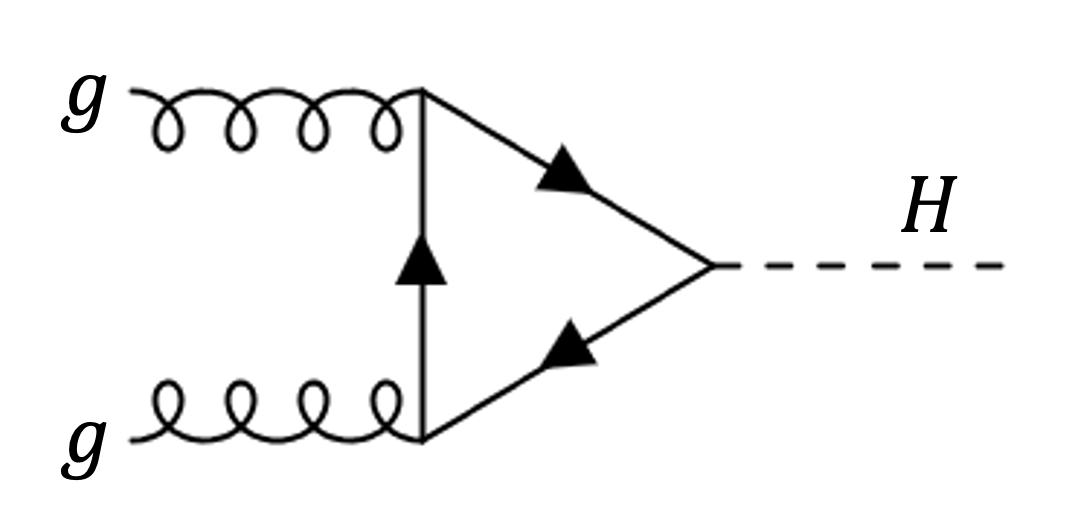
\includegraphics[width=0.24\textwidth]{Images/Theory/ggH.png}
    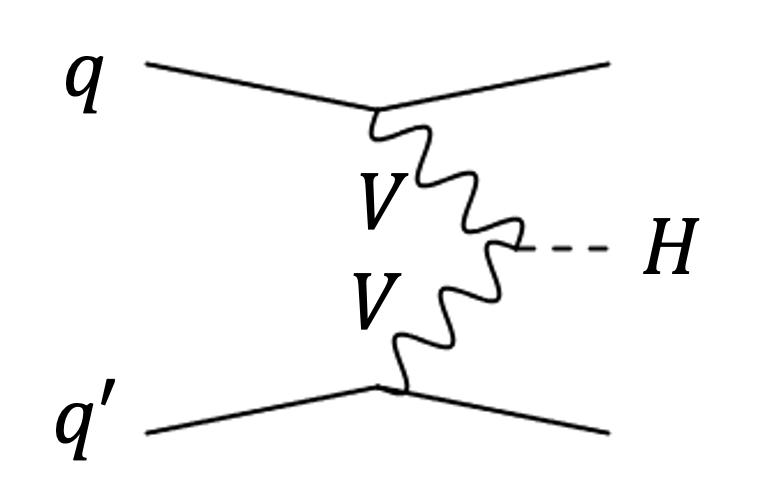
\includegraphics[width=0.24\textwidth]{Images/Theory/vvH.png}
    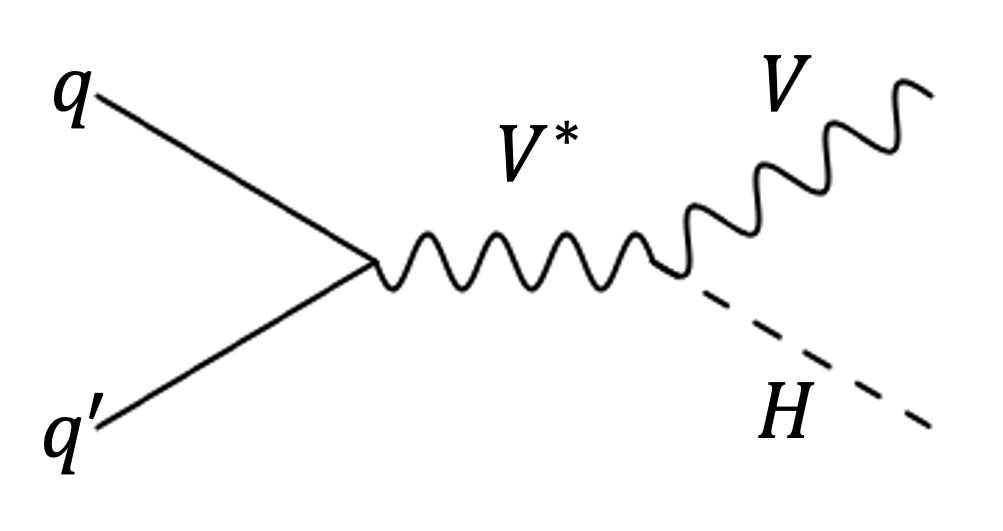
\includegraphics[width=0.24\textwidth]{Images/Theory/vh.png}
    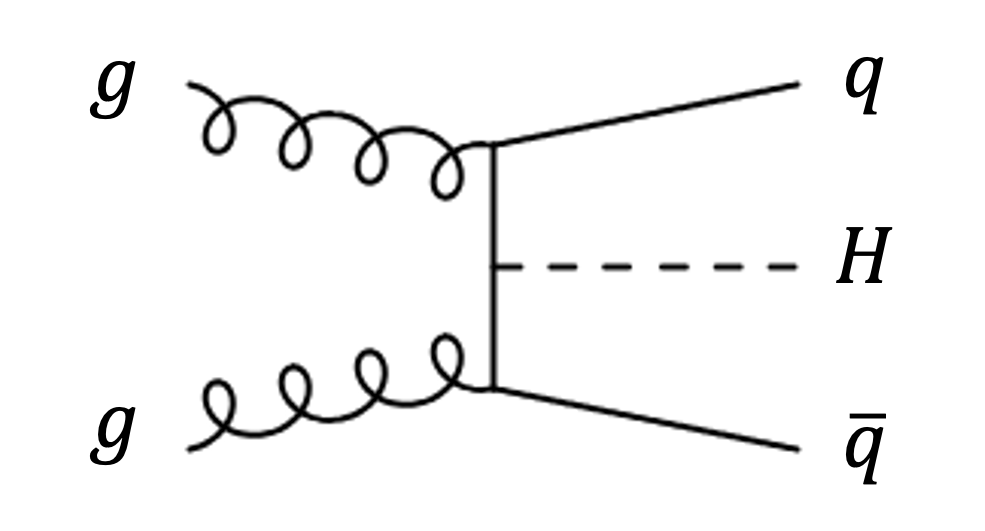
\includegraphics[width=0.24\textwidth]{Images/Theory/qqH.png}
    \caption{The leading order Feynman diagrams for Higgs production at the LHC, from left to right: gluon-gluon fusion ($ggF$), vector boson $V$ fusion ($VBF$), associated production with a vector boson ($VH$), and associated production with a $q\bar{q}$ pair ($q\bar{q}H$).}
    \label{fig:prodH}
\end{figure}

The dependency of the Higgs boson production from proton-proton collisions at $\sqrt{s} = 13$ TeV are represented in the left of Figure~\ref{fig:prodH} as a function of the Higgs boson mass $m_H$. The total width of the \gls{sm} Higgs boson is $\Gamma_H = 4$ MeV, implying a short lifetime of $\tau_H ~ 10^{-22}$ $s$ and restricting measurement to its decay products. The decay branching ratios are displayed in the right of the figure, with decays to heavier particles favoured due to the proportionality of the Higgs coupling strength to the mass. Decays to the massless gluons $g$ and photons $\gamma$ are possible thanks to intermediate quark loops, similarly to $ggF$. Relative decay rates are quantified by their branching ratio $BR$ as
\begin{equation}
    BR(H \rightarrow X) = \frac{\Gamma(H\rightarrow X)}{\Gamma_H}
\end{equation},
where the total Higgs width $\Gamma_H$ is the sum of all partial decay width $\Gamma(H\rightarrow X)$, for all possible $X$. The right of Figure~\ref{fig:prodH} displays the \gls{sm} Higgs branching ratio at $\sqrt{s} = 13$ TeV. The most likely decay mode is to a pair $b\bar{b}$ ($BR \approx 58$ \%), followed by the decay to a $WW$ pair ($BR \approx 21$ \%). The decay branching ratios are displayed in the right of the figure, with decays to heavier particles favoured due to the proportionality of the Higgs coupling strength to the mass.

\begin{figure}[h!]
    \center
    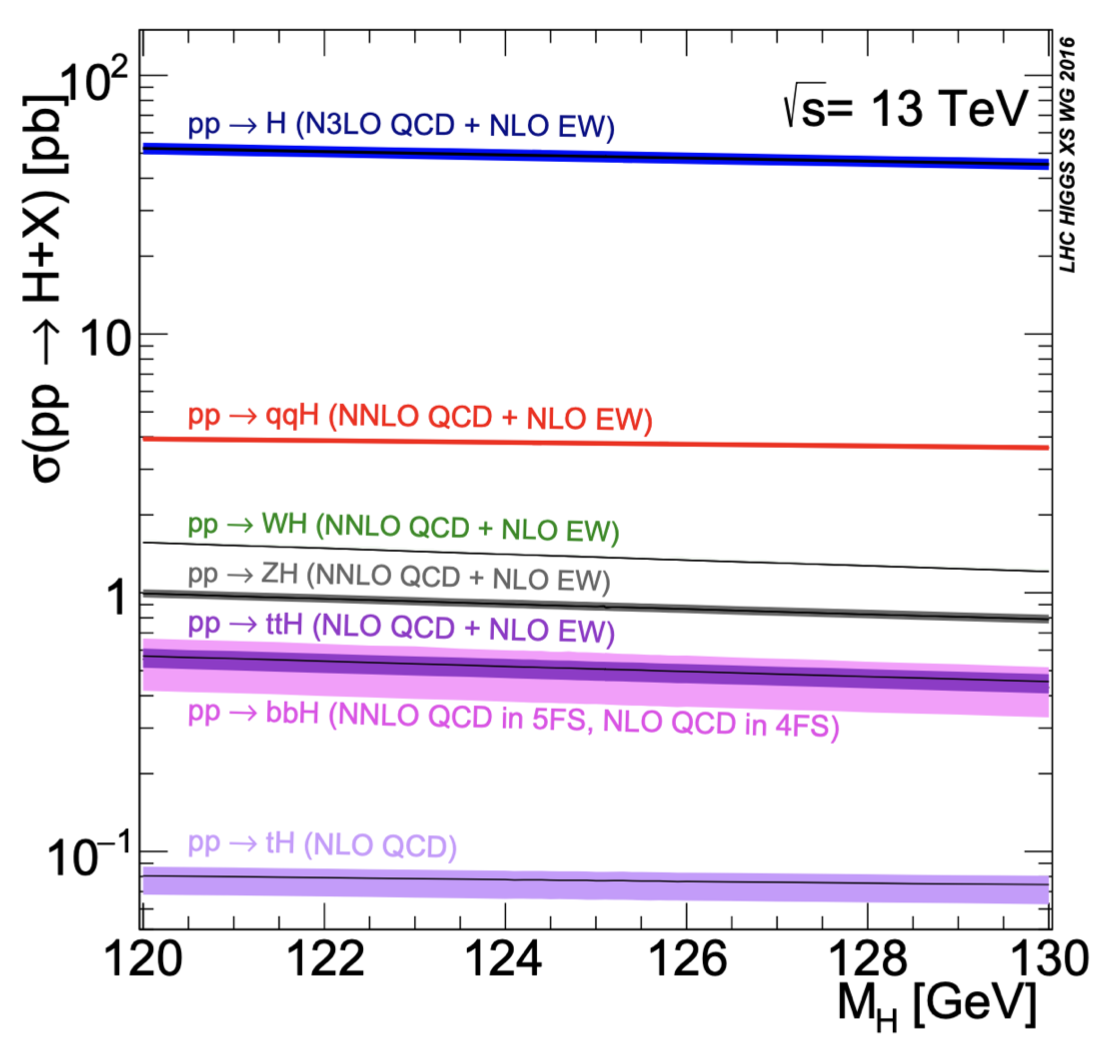
\includegraphics[width=0.48\textwidth]{Images/Theory/prodHiggs.png}
    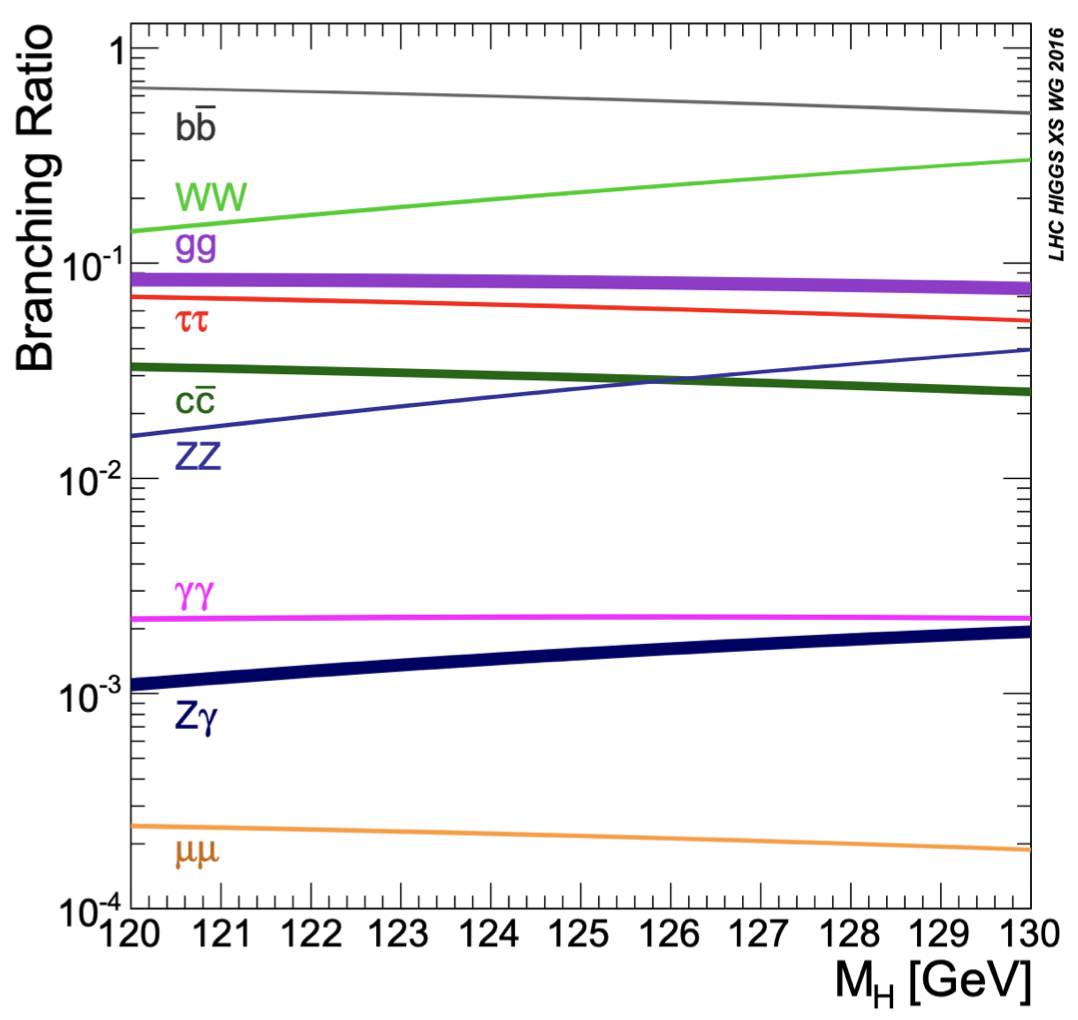
\includegraphics[width=0.48\textwidth]{Images/Theory/decayHiggs.png}
    \caption{The Standard Model production cross-sections from proton-proton collisions (left) and decay branching ratio (right) of the Higgs boson as a function of $m_H$, at $\sqrt{s} = 13$ TeV.}
    \label{fig:prodH}
\end{figure}





%%%

In figure \ref{particlesSM}, the two top left purple rows list \textit{quarks} (declined into different \textit{flavours}, such as the up $u$ and the down $d$), the only elementary fermions sensitive to the strong interaction. This mechanism is described by the quantum field theory of \gls{qcd}. \textit{Colour} stands for the elementary strong charge and comes in three variants: blue, red, and green. The mediator of this interaction, called the \textit{gluon} ($g$), is itself colour-charged (with two charges in fact) and massless, which has a deep implication on the behaviour of quarks and gluons called \textit{colour-confinement}. This effect can be (approximately) understood as the strength of the colour-bound increasing with the distance of separation, forcing coloured-components to aggregate. The image of a string is often mentioned to describe this particular type of bond. Because opposite colours or the combination of all colours neutralise the charge, they combine to form \textit{colourless} objects called \textit{hadrons} (Greek for ``massive'', used as an opposition to \textit{leptons}, meaning ``light'' and corresponding to the two bottom left rows of figure \ref{particlesSM}). These aggregated states consist in \textit{mesons} (a quark and an antiquark, such as the pion - Greek for ``intermediate''), \textit{baryons} (a set of three quarks, such as the proton - Greek for ``heavy''), and more exotic compounds, such as \textit{tetraquarks} (a set of four quarks). The process forcing the combination of coloured elementary particles into colourless objects is called \textit{hadronisation}. A complete theoretical description of this mechanism has not yet been fully derived, with several phenomenological approaches widely adopted \cite{Looking_Inside_Jet}. 

Given that both quarks and gluons have a colour charge, colour-confinement forces them to combine with other coloured matter to form colourless aggregates. Note that where that matter comes from precisely is still an active subject of investigation. In the \gls{sm}, these external particles are presumed to emanate from quark-antiquark pairs spontaneously created from the vacuum. The result of their hadronisation is a cascade of combinations and decays that form a tight cone of particles around the trajectory of the hadronising particle. Indeed, by the law of energy-momentum conservation, the momentum $\vec{p}$ of the initial particle is shared between the final state constituents, hence the general global orientation. Such a conic structure of decays is called a \textit{jet}. A real ATLAS event with multiple jets is represented in figure \ref{multiJet}. The process of gathering final state constituents to reconstruct the global jet is called \textit{clustering} \cite{Looking_Inside_Jet}. It is performed by \textit{clustering algorithms} with the whole history of decays organised into a \textit{factorisation tree}, as discussed in more details in section \ref{Section:ProcData}.

%\begin{figure}[!h]
%\centering
%\includegraphics[scale = 0.3]{Images/MultiJetEventDisplay.png}
%\caption[A multijet event in the ATLAS detector]{A multijet event in the ATLAS detector %\cite{JetImage}. The green and yellow volumes represent energy deposits in specific %parts of the detector (ECAL and HCAL). The small orange curves in the centre are %individual particle tracks. Note how many of them are grouped behind each large energy %deposit, an evident sign of the presence of a jet. }
%\label{multiJet}
%\end{figure}

To observe quark and gluon jets as well as any other animal of this particle zoo, massive accelerator complexes and detector systems were assembled. This short introduction focuses on the ATLAS Experiment at CERN, since this project is calibrated to their data input. In Physics, energy and (inverse) length are connected, as suggested by the famous Planck-Einstein relation $E = \frac{h \, c}{\lambda}$, relating the energy $E$ to Planck's constant $h$, the speed of light in vacuum $c$ and the wavelength $\lambda$. To observe or, equivalently, to measure requires to reach a wavelength of the size of the investigated objects and therefor the right energy. The smaller the object, the larger the energy required. The interest of accelerators is precisely to increase the kinetic energy of components before ``releasing'' their content through collisions but, more generally speaking, interactions. New elements are produced from the decay of the initial particles that unveil the processes ruling Physics at the energy investigated. Most accelerators, such as the CERN's \gls{lhc}, exploit a circular shape to keep the beams of charged particles, typically gathered into bunches, in a closed trajectory while their speed (and hence kinetic energy) is increased with each revolution by the use of radiofrequency cavities. This device generates an oscillating electromagnetic field synchronised with the evolving revolution frequency of the bunches to accelerate them. The beams are constrained to their expected trajectory by powerful magnetic systems. Different geometries, such as dipoles and quadrupoles are used to monitor, control, and shape the extent of the bunches. The \gls{lhc} is only the last ring in a complex chain of accelerators, as suggested in the diagram of the CERN operation presented in figure \ref{CernAccSys}. It operates with pre-accelerated protons or \textit{ions} (atoms or molecules with a net electrical charge). 

\begin{figure}[!h]
\centering
\hspace*{-0.5in}
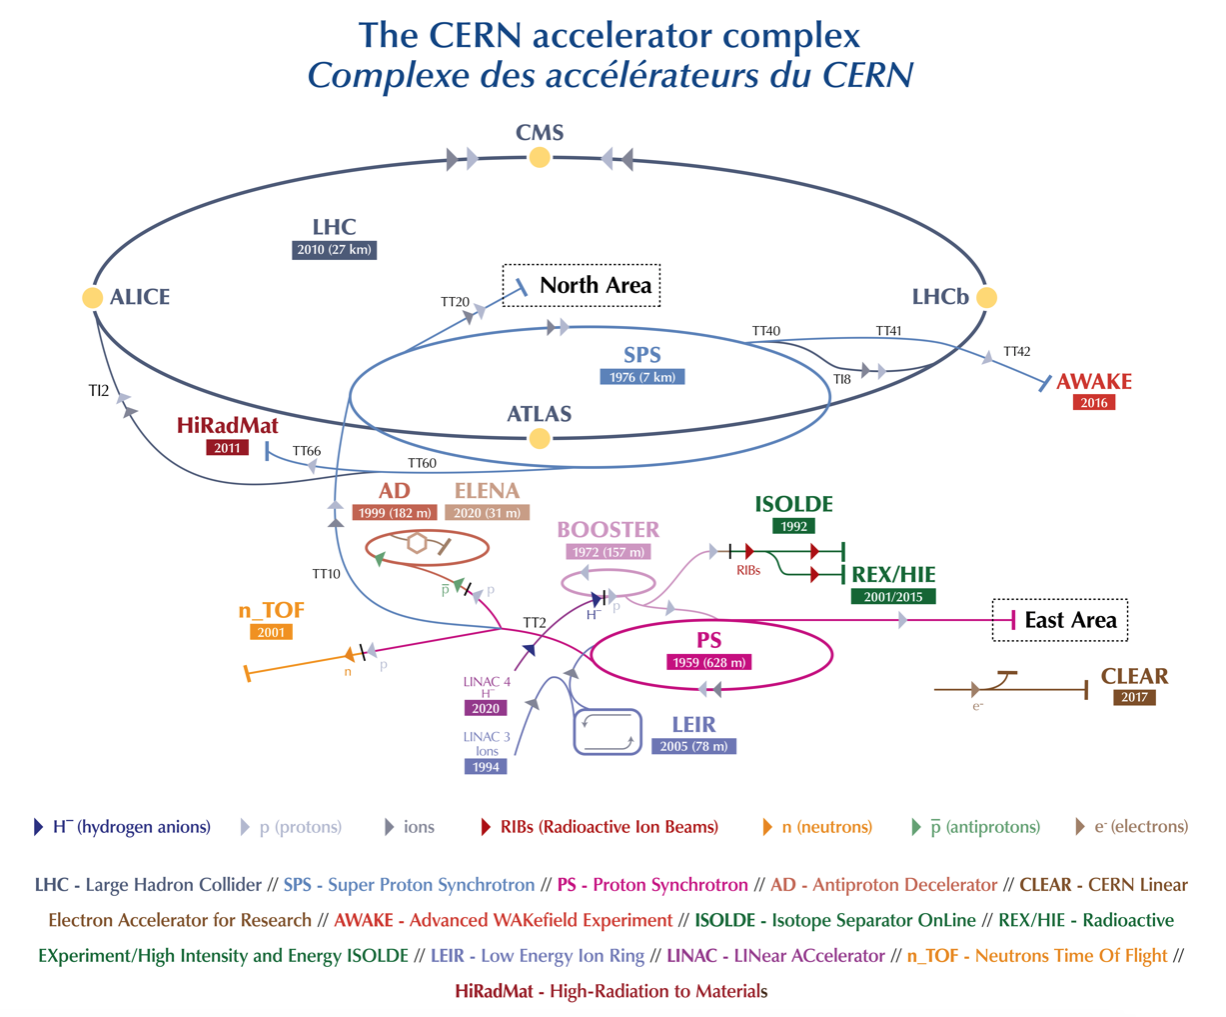
\includegraphics[scale = 0.4]{Images/ATLAS/cernAcc}
\caption[Accelerator complex of CERN in 2019]{The accelerator complex of CERN in 2019 \cite{Mobs:2684277}. The LHC is the top dark blue ring.}
\label{CernAccSys}
\end{figure}
\newpage
Along their trajectory, two different beams can collide at a controlled \textit{\gls{ip}}. The word \textit{event} is used to encompass all information and processes emanating from the collision of two bunches (all collisions within a 25 ns period). For the purpose of this project, the collided elements in the two beams are protons at a centre of mass energy of 13 TeV, where 1 TeV = 1000 GeV. At these energies, the constituents of protons, as perceived by observing their decay, do not match the often presented and simplified three quarks picture (2 $u$ and 1 $d$). They are made of a probabilistic set of constituents called \textit{partons}. \textit{Parton distribution functions} were phenomenologically derived to quantify the probability distribution of observing a given parton at a given momentum transfer due to the interaction undergone \cite{pdfLHC}. In a sense, the content of a proton is governed by a probability distribution depending on the energy at which the proton is observed. Physicists analyse the constituents of matter arising from the collision by building giant detectors around this particular location. The ATLAS collaboration uses a cylindrically shaped multi-layered detector that is 45 m long with a diameter of 26 m and sitting in a cavern 100 m below ground, as presented in figure \ref{AtlasDec}.

\begin{figure}[!h]
\centering
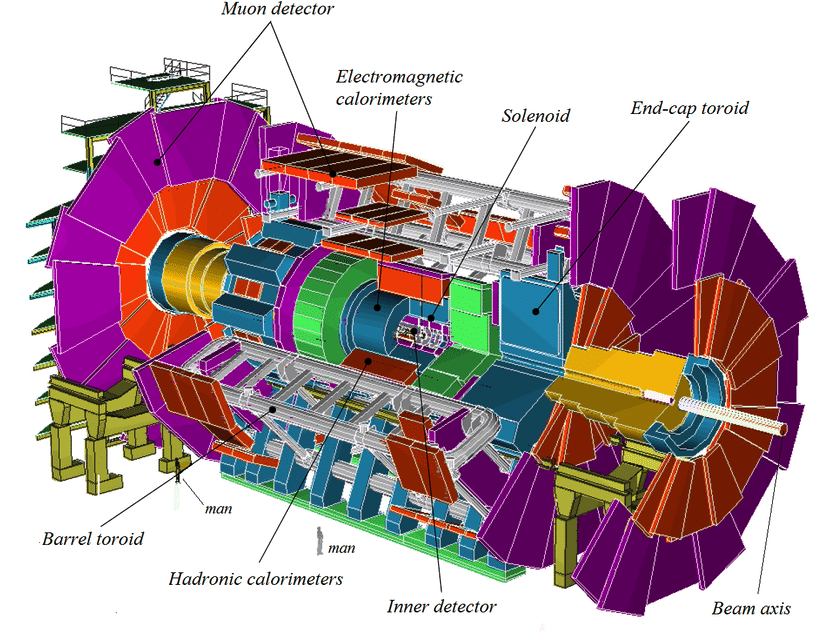
\includegraphics[scale = 0.5]{Images/ATLAS/Atlas.png}
\caption[Schema of the ATLAS detector]{Schema of the ATLAS detector \cite{AtlasWeb}.}
\label{AtlasDec}
\end{figure}

Such a detector is far more versatile than needed for the present project. This short presentation focuses on its essential components. Following a radius from the \gls{ip} (in the centre of the detector) towards the exterior, the main elements encountered are \cite{AtlasInstruDec}:
\begin{itemize}
\item An inner detector: different technologies are deployed to be sensitive to the presence of charged particles in active cells. It allows the reconstruction of a \textit{track} (a path) for electrically charged particles going through its layers, lending to the device the name of \textit{track detector} or \textit{tracker}. A variety of algorithms are employed in the ALTAS experiment to fit a track to a set of hits. A \textit{hit} is a localised deposit of energy, usually in a tracker or a calorimeter cell. A point from which new tracks emerge is called a \textit{vertex}, with the \textit{\gls{pv}} being the main vertex of the event, from which most of the interesting tracks come. 
\item A solenoid: a large cylindrical magnet releasing a magnetic field parallel to the axis of the cylinder, along the beamline. It has the effect of curving the trajectory of charged particles, as dictated by the famous Lorentz force $\vec{F} = q \vec{v} \times \vec{B} + q \vec{E}$, $q$ being the charge of the particle, $\vec{v}$ its velocity, and where $\vec{B}$, the magnetic flux density, and $\vec{E}$, the electrical field, are taken at the position of the particle. A curved trajectory in this fixed magnetic field reveals the electric charge of a particle (since a flip of $q$ changes the direction of rotation for a given $\vec{v}$). Another advantage of curving the trajectory of a charged particle with a fixed magnetic field comes from the ability to estimate its momentum $\vec{p}$ by measuring the radius of curvature $\rho$ with the relation $p = qB \rho$. Note that for a given $p$, one can control $\rho$ by adapting $B$: this is exactly what the magnetic system of the accelerator does to constrain the bunches to their expected trajectories. 
\item Calorimeters: electromagnetic (ECAL, for electrons, positrons, and photons) and hadronic (HCAL, for hadrons) calorimeters are large active volumes which purpose is to collect (most of) the energy of a passing particle. The calorimeters are structured into cells (separated into a forward region, called \textit{endcaps}, and a central region, called the \textit{barrel}). A cell collecting an amount of energy over a certain threshold is recorded as a hit. In the ATLAS experiment, groups of cells thus triggered are clustered into larger structures called \textit{topoclusters}, for topological clusters.
\end{itemize}

The reference frame adopted in the present work is introduced in figure \ref{CoorSystem}, with the two angles being the polar angle $\theta$ and the azimuthal angle $\phi$. The $x$-axis points towards the centre of the \gls{lhc} ring, the $z$-axis is taken along the beamline, and the $y$-axis closes the basis, so that the system $x-y-z$ is right-handed. Variables living in the $x-y$ plane are referred to as \textit{transversal} and added the subscript ``$_T$''. For example, the energy projected in the transverse plane is called $E_T$ and the projection of momentum $\vec{p}$ in the $x-y$ plane is $\vec{p}_T$ with a magnitude of $p_T$, the latter being a particularly important variable in \gls{hep}. Instead of the polar angle $\theta$, one often uses the pseudo-rapidity $\eta = - \log \left( \tan \frac{\theta}{2} \right)$ that maps the $\theta$ range of $[0, \pi ]$ to $[ -\infty, \infty ]$. This transformation is motivated in ultra-relativistic Physics by the closeness of the pseudo-rapidity to the notion of rapidity. The two notions are in fact equal for massless particles. Note that there is a natural limit to the range of $\eta$ to which the detector is sensitive since, at values of $\theta$ closed to 0 or $\pi$, the particle is still inside the beam pipe and cannot be detected. The geometrical ($\eta$) and dynamical ($p_T$) limitation of events observable due to the limits of the detector is called the \textit{acceptance}. It depends on the object being studied, as different subdetectors may be involved in gathering information to identify it. A typical acceptance range for $\eta$ is the range $[-3, 3]$. 

%\begin{figure}[!h]
%\centering
%\includegraphics[scale = 0.65]{Images/Coordinate_system.png}
%\caption[Coordinate system used by the ATLAS experiment]{The coordinate system used by %the ATLAS experiment. The $x$-axis points towards the centre of the LHC and the %$z$-axis is along the beamline (p symbolises a proton). For a particle of velocity $\vec%{v}$, $\theta$ is the polar angle (between $\vec{v}$ and the $z$-axis) and $\phi$ the %azimuthal angle (between the projection of $\vec{v}$ on the $x-y$ plane and the %$x$-axis). }
%\label{CoorSystem}
%\end{figure}

In operation, the enormous rate of collisions occurring in the centre of the detector (close to 40 MHz) causes a data transfer bottleneck. A set of filters must be employed to restrict data processing to events deemed of interest. These filters are called \textit{triggers} and are implemented by a hierarchical setup of electronic devices, for the lower level, and numerical methods, for the higher one, to progressively reduce the rate of events. The raw data collected that passes all steps of the triggers can then be stored in giant databases. Several layers of processing are applied to reconstruct higher-level variables, such as the energy, the mass of a particle, the tracks, and, most importantly here, the identity or \textit{tag} of the particle (e.g., gluon or quark), from low-level information, such as hits in the tracker and deposit in the calorimeter cells. Assigning a label to a particle is called \textit{tagging}. A hierarchy of increasingly processed databases for different signal regions (regions with a predominance of a specific sort of events or particles, depending on the trigger setup used when collecting the data) is then accessible to physicists. 

To analyse the data and extract the above relevant information, several techniques are employed. As the probabilistic nature of quantum physics forbids exact event-by-event analysis, one is forced to consider distributions of observables (for example the invariant mass, equal to the energy in the centre of mass of the collision). Given this stochastic aspect, \gls{mc} methods are the natural simulation tool to produce physical events as dictated by the relevant theory: this is called the \textit{generated level} \cite{Ay:2010zza}. \gls{mc} methods were in fact initially developed for this purpose, although in a more military context. The simulated events can then be passed through another layer of simulation to include the act of detection, bringing them to the \textit{reconstructed level}. For example, when two bunches collide, the detector records a set of simultaneous and overlapping events, an effect known as \textit{\gls{pu}} that needs to be added to simulations. Many reconstructed events thus produced are agglomerated into distributions, to be compared to the measured ones. Consequently, theoretical predictions can be tested against the recorded information, to search for either agreement or deviation. This is a scientifically highly efficient albeit computationally intensive process that has favoured the common pulling of resources into a worldwide computing grid and, most notably, the Web, created at CERN in 1989 and made public in 1993. 

\section{Motivation and Open Questions}\label{Section:Mot}
The previous sections introduced the landscape of the Physics experiment. The intense efforts devoted to these gigantic experiments come from the need to perform precise tests of the Standard Model and uncover traces of new Physics. For many reasons, the \gls{sm} cannot be the final theory. For example, it already fails to include gravity. Joining this interaction with the other ones is challenging, given it is extremely weak at the quantum level and only becomes somewhat significant at larger scales, due to the positive aggregation of matter. The ambitious research programme of the Particle Physics community requires several characteristics \cite{BSM_HL_LHC}: 
\begin{itemize}
\item Many events, to reduce the statistical incertitude.
\item High energies, to increase the range of processes that can occur in a collision. Currently, the average centre of mass energy of proton-proton events in the \gls{lhc} is of about 13 TeV. 
\item Fine granularity and precise methods, to improve the quality of the collected data, reconstruct more events, implement better selections, reduce the data transfer bottleneck, improve the accuracy by finer track reconstruction, and have better-aggregated information.
\end{itemize}
The first two points are regularly improved by upgrades of the components of the intricate experimental system of the CERN accelerator complex and the ATLAS detector. The final point can greatly benefit from machine learning. This has attracted a community-wide interest for these methods, with many applications already derived, particularly in classification and reconstruction (such as track fitting and pile-up removal) \cite{Deep_Learning_HEP}. 

One such effort that is of paramount importance to the advancement of research in Particle Physics is the ability to identify and discriminate jets, and in particular those associated with quarks and gluons. These objects are indeed a by-product of many different physical processes. They leave very noticeable patterns in the different subdetectors, turning them into natural and evident clues to hunt specific signals. Better \gls{qcd} and \gls{sm} measurements as well as improved and new searches for exotic physics would be the prize of a significant increase in efficiency \cite{Search_HEP_Deep_Learning}. Specifically related to the task of quark versus gluon jet discrimination, two promising analyses that would benefit greatly from an improved classifier are \cite{QG_ML_vs_Detector}:
\begin{enumerate}
\item Searches for mono-jet of dark matter in a gluon-dominated signal.
\item Searches for dijet resonances in a quark-dominated signal.
\end{enumerate}

The history of machine learning in the context of High Energy Physics is already long, beginning with \gls{mva} in the early 2000s \cite{Bhat:2010zz} to recent deep learning applications. Most importantly, in the context of jet tagging, recently explored techniques include:
\begin{itemize}
\item \glspl{bdt}: the reference method, most commonly used given its flexibility and ease of training for a relatively good performance when fed ``highly-engineered'' physical inputs \cite{QG_ML_vs_Detector, QG_Tagging_Charged}.
\item \glspl{dnn}: their performance is usually comparable to \glspl{bdt}'s, or marginally better \cite{Definition_QGJets}. It also requires engineered inputs, for competitive efficiency. 
\item Image analysis: the calorimeter surrounding the interaction point offers a natural 3D image of the jet energy deposits. This can and has been exploited in several \gls{cnn} models. The performance obtained is however not state-of-the-art for quark versus gluon discrimination, even when combined with inside information from the tracker, but it does perform slightly better than basic \glspl{bdt}'s and \glspl{dnn}'s using typical jet information \cite{QG_JET_Tagging_Image}. The significant advantage of these methods resides in the possibility to deploy them in triggers, as they only use low-level information (calorimeter hits). 
\item Junipr: a framework for unsupervised learning deploying a \gls{rnn} around a leading order model of Physics to learn the probability distribution underlying the data \cite{Junipr}. Most observables in quantum field theory are derived through perturbation theory to a certain degree or order, with the leading order being the first term. The Junipr framework offers the possibility of performing a likelihood ratio test to discriminate between different learnt distributions (from simulations) corresponding to different types of jets. Furthermore, the probabilistic model learnt when scaffolded around a factorisation tree (a tree giving a successive order to decays leading to the final state particles observed) is interpretable. In 2019, the method was proven state-of-the-art for quark versus gluon jet discrimination on a set of simulations at the generated level \cite{JUNIPER_Discrimination}. Broadly, the method relies on \gls{rnn} to learn from the succession of decays characteristic of a specific type of jet \cite{QG_RNN_tagging}. Given these qualities, the Junipr approach is the chosen paradigm for this project and is described thoroughly in section \ref{Juniprintro}.
\item Particle cloud: an adaption of point cloud considering a jet as an unordered list of final state particles. When combined with Dynamic Graph \gls{cnn} to perform complex convolution operations on the graph of final state particles, the method can achieve good performance for jet tagging problems \cite{ParticleNet}. This approach exploits recent progresses in \gls{gnn} \cite{Survey_GNN}.
\item Energy Flow Network: this method produces a set of highly-engineered features called \textit{energy flow polynomials}. They constitute a complete set of jet substructure observables, forming a discrete basis \cite{Basis_Jet_Energy_Flow}. This information can be passed to any of the previously mentioned methods (linear classifier, \gls{bdt}, \gls{dnn}, \gls{cnn}, ...) to improve its performance in the tagging and discrimination tasks \cite{Komiske2019EnergyFN, Number_Charged_Jet}. 
\item Weakly supervised learning: several papers have suggested that this learning paradigm could prove ``more physical'' \cite{Definition_QGJets}. Indeed, the assignment of a jet as emanating from a quark or a gluon parton is an inherently phenomenological one, as it does not correspond to any real physical process. The quantum world is far more complicated than the simple image this may suggest, as the contents of a proton themselves are a probabilistic mix and jets emanate from interactions within these distributions (the previously introduced parton distribution functions). Jets are assigned such a label when their orientation corresponds to that of a \textit{mother} parton momentum. What is typically called a quark or gluon jet is a specific object possessing its own properties and emanating from distinct scenarios. Therefore, rather than learning with exact labels, it has been proposed to pursue discrimination between quark- or gluon-rich distributions collected directly from the data, made of impure samples \cite{WS_taxonomy, WS_Classification_HEP, Classification_Impure_samples, Classification_no_Label_HEP}.
\end{itemize}

These various methods have been applied with different levels of success to the task of jet tagging using information from physical simulations. However, most of them are not considered in the context of a specific measuring device, as they are restricted to \textit{generated} level simulations. Measuring distorts to a certain degree (depending on the measured variables, the state of the detector at the time, ...) the underlying distribution to bring it to the \textit{reconstructed} level. It is an unavoidable consequence of interacting with the Universe at our scale. The extra-layer of simulation required to mimic the act of detection, introducing variance and blurring the descriptive power of observables, has to be accounted for when considering the level of a certain experiment, confronted to a specific way of collecting data. The aim of this project, described in the next section, is to confront a selection of these methods to the reality of the ATLAS experiment at CERN. 

\section{Objectives and Organisation}\label{Section:Obj}
From the previous section, one can conclude that there are three main ways of representing a jet: 
\begin{enumerate}
\item As a physical object, with observables describing it, such as its width, and number of constituent particles. This leads to common methods, such as \glspl{dnn} and \glspl{bdt}.
\item As an image: whether solely from the calorimeter or combined with track and other information, offering a natural ground for \glspl{cnn}. 
\item As a succession of branchings, whether ordered (factorisation tree) or unordered (particle cloud). This gives a relational point-of-view adapted to \glspl{rnn} and \glspl{gnn}.
\end{enumerate}
This project implements \glspl{dnn} and \glspl{bdt} models for benchmark and the Junipr approach from the paradigm of recurrent learning to the specific case of the ATLAS experiment. Two main research questions are explored with this subset of models: 
\begin{enumerate}
\item Is it possible to efficiently discriminate quark and gluon jets based on the low-level information delivered by the calorimeters of the ATLAS experiment? For this purpose, Junipr models are adapted to work with topocluster momenta. Junipr is chosen as it obtains state-of-the-art result on generated level simulations.
\item Is a Junipr approach competitive compared to commonly used methods when working at the reconstructed level? For this purpose, \glspl{dnn} and \glspl{bdt} models on high-level variable of reconstructed simulations are implemented. These models were chosen as they are quite common in the field and exploit engineered variables. They thus provide a natural benchmark to analyse the results of Junipr. 
\end{enumerate}
The main novel contribution of this work is to implement the Junipr model for fully \textit{reconstructed} simulations, which are intrinsically noisier than generated-level data. Indeed, reconstructed-level data suffers from the limited precision of the detecting device, pile-up, and competing processes (both reducible, if they possess different final states, and irreducible, if they do not). The second important contribution is to develop an efficient quark versus gluon jet classifier restricting to \textit{low-level} information from the detector. This final constraint, vastly complicating the task given the lower information content, is motivated by the following points: 
\begin{itemize}
\item This kind of information is that directly gathered by the detector and, therefore, the first one accessible: exploiting it efficiently is vital in the context of triggering. A precise algorithm, trained offline, could quickly perform an intelligent online selection of interesting events. 
\item Low-level information has a geometrical nature (such as the energy deposit and track hits) due to the extent and localisation of detector cells and, to a certain degree, a recurrent one (track combination and vertices, points where new tracks emanate, radiate in a tree structure from their initial point, the \gls{pv}). Many advanced \gls{ml} techniques from the previous section can exploit these patterns. 
\end{itemize}

This project is an interdisciplinary effort between the Computer Science and Particle Physics departments of the University of Oxford. The objective of this work is to serve as a concrete basis for future physics analyses by assessing the potential of new specific computational tools based on advanced \gls{ml}. Interesting steps such as interpreting the distributions obtained (except when assessing the quality of results) or searching for specific signals involving quark and/or gluon jets are not included in the present dissertation and are left for future research. Given the COVID-19 pandemic in 2020, the entire work was carried out remotely and contacts with supervisors were restricted to mostly weekly Teams meetings (sometimes at a higher frequency with Aaron O'Neill during the stages concerned with collecting the data). This has not caused any significant issues. Indeed, the CERN community, being spread all around the globe, is used to deal with such communication restrictions and have thus developed an organisational structure appropriate for remote access.

\vspace{3.5cm}

\begin{tcolorbox}[colback=oxfordblue!5,colframe=blue!40!black,title=Summary of the Chapter]
{This chapter introduces the physical context of the project. Quarks and gluons are elementary particles from the Standard Model of Particle Physics. Having a colour charge, they are sensitive to the effects described by \gls{qcd} and hadronise to form colour-less objects. This process generates large structures of successive decays called \textit{jets} and leaves a remarkable pattern in the detector of the ATLAS experiment, based on the \gls{lhc} at CERN. Jets provide a useful tool to search for and isolate specific signals in the collected data to compare to theoretical predictions. A review of current methods introduces different machine learning-based techniques to discriminate quark from gluon jets. Among them, the Junipr framework is the most promising option, given it leads to state-of-the-art performance at the generated level and is interpretable when founded upon a physical factorisation model. This project studies an adaptation of the Junipr approach to use low-level calorimeter information to improve the accuracy at the reconstructed level of the quark versus gluon jet discrimination task. \gls{bdt} and \gls{dnn} models serve as benchmarks, given their popularity in the field and reliance on high-level variables.}
\end{tcolorbox}
